
\chapter{Multi-Behavior Decision-Making Strategy}
\label{Chap05}
\begin{abstract}
    This chapter is dedicated to draw the details related to the decision-making level part of the proposed Cooperative Multi-Controller Architecture (C-MCA) for MVS performing on-ramp merging on highway, thus under the prisme of safety, passenger comfort, and energy efficiency. The proposed multi-behavior selection strategy predicts the safety assessment during the merging scenario based on a nominal behavior of the MVS. Based on the safety criterion, the optimal behavior of the MVS is chosen, either to perform the merging in a nominal manner, or to overcome a conflicting situation in a cooperative manner \footnote{The detailed contributions in this chapter have been the subject of the following publications  \hyperlink{ITSC23}{ITSC'23}, \hyperlink{MMAR23}{MMAR'23} and \hyperlink{VAMS23}{VAMS'23}.}.
    
\end{abstract}


\textbf{Contents}
\vspace{0.15cm}
\hline
\hspace{2cm}
\localtableofcontents
\hspace{2cm}
\hline
\hspace{2cm}



% il faut plus commencer par rappeler ce qu'on a vu avant et comment ce qu'on a vu avant et bien il sera utilisé ici. 
The decision-making level part of the proposed Cooperative Multi-Controller Architecture (C-MCA) for MVS was designed to answer three main questions: 
\begin{enumerate}
    \item What is the nominal dynamic for each vehicle part of the MVS to perform the merging?%\footnote{Nominal dynamic: this term is used in this PhD work in order to describe the dynamic of the vehicle that permits to optimize its priorities.}?

    \item How to predict the potential conflicting merging scenarios when the vehicles are operated by their nominal behavior?

    \item How to solve the conflicting merging when occurred, with minimum changes imposed to the nominal behavior, while taking advantage of the MVS cooperative ability? 
\end{enumerate}





\\



The decision-making level employs a multi-behavior decision-making strategy. Based on the collision risk metric, the proposed strategy depicted in Figure \ref{fig:behavior_selection},  has the responsibility of switching between two embedded behaviors. The first objective of this chapter is to delve into the selection strategy used by the decision-making-level. In Section \ref{sec:Multi-behavior_selection_strategy}, the details of the selection strategy are given. The second objective of this chapter is to delve into the details of the nominal behavior through Section \ref{sec:The_nominal_mode}. Additionally, the details the of the cooperative behavior are discussed in Section \ref{sec:Cooperative_mode}. Where the concept of the passing sequence is explained, and an appropriate passing sequence selection approach is proposed. 

       \begin{figure}[!h]
        \centering 
        \includegraphics[width=10cm,height=18cm,keepaspectratio]{chapters/Chapitre_6/Figures/Architecture.png}
        %\vspace{-2.3mm}
        \caption{The proposed multi-mode behavior selection level, part of the overall C-MCA (cf. Figure \ref{fig:C-MCA})}
        \label{fig:behavior_selection}
        %\vspace{-5mm}
        \end{figure}




The performance of the multi-behavior decision-making strategy, serving as the decision-making level within the C-MCA, is assessed through simulations detailed in both: the Section \ref{sec:nominal_simulation_results} for the nominal behavior and in Section \ref{sec:Simulation_Results} for the cooperative behavior. 



 \section{Multi-behavior selection strategy}\label{sec:Multi-behavior_selection_strategy}










One of the central objectives of the proposed C-MCA is to ensure that the merging maneuver of the MVS is executed with appropriate dynamics while prioritizing the safety requirements. This involves the design of the MVS's nominal behavior, which is focused on the optimization of the vehicles' dynamics in alignment with their individual objectives (cf. Section \ref{sec:The_nominal_mode}). 

To initiate the behavior selection process, the first step is to predict the nominal behavior of each vehicle within the MVS (cf. Figure \ref{fig:behavior_selection}). Following the nominal behavior generation strategy, this prediction process also extends to forecasting the distances between the vehicles throughout the merging maneuver. This step is crucial in identifying potential collision risks among the vehicles (cf. Figure \ref{fig:behavior_selection}). 


     % \begin{figure}[!h]
     %    \centering 
     %    \includegraphics[width=7cm,height=18cm,keepaspectratio]{chapters/Chapitre_6/SelectionMode.pdf}
     %    %\vspace{-2.3mm}
     %    \caption{The proposed multi-behavior decision making system}
     %    \label{fig:multi-behavior selection system}
     %    %\vspace{-5mm}
     %    \end{figure}



Subsequently, the safety metric is assessed under two main scenarios, as illustrated in Figure \ref{fig:behavior_selection}. In the first scenario, which corresponds to the absence of predicted collisions within the merging zone.Triggered by the nominal behavior predictions, the decision is made to activate the nominal behavior. It is important to note that, even when the nominal behavior is initially activated, the safety criterion is continuously monitored through a feedback loop. If, at any point, the safety criterion predicts a collision within the merging zone, the decision-making level promptly activates the cooperative behavior to avert and avoid the collision risk. In the second scenario, where a predicted collision risk is present, the C-MCA activates the cooperative behavior (cf. Section \ref{sec:Cooperative_mode}). 

In the following section, the details related to the nominal behavior are given along with corresponding simulation results. 

















\section{Nominal behavior} \label{sec:The_nominal_mode}

This section is dedicated to draw the explanation related to the nominal behavior part of the multi-behavior decision-making implemented in the C-MCA. Simulation results on an on-ramp merging scenario performed by the nominal behavior are presented in this section. 

\subsection{Overview of the nominal behavior part of the C-MCA}

The goal of the nominal mode is to perform the merging maneuver while optimizing each vehicle's dynamics w.r.t. their individual goals (cf. Figure \ref{fig:illustration_nominal_behavior}). For instance, the highway vehicles have an already established highway dynamics, thus their aim is to keep tracking the latter. As for the merging vehicle, it aims to perform the merging maneuver while minimizing the merging time, and to not modify a lot its planned velocity (generally depending on the road velocity limitation). 

This mode takes the assumption of a free merging zone. Consequently, no conflicting scenario is considered. It is important to note that this assumption permits to focus only on the vehicles' dynamics, such as their individual goals are satisfied. Consequently, the safety criterion when generating the nominal mode is assessed by the decision-making level. 


The nominal behavior of the highway vehicles consists of their initial dynamics through the merging maneuver. In fact, the highway vehicles have an already established dynamic when traveling in the highway (cf. Figure \ref{fig:illustration_nominal_behavior}) (in general calibrated w.r.t. the maximum authorized highway velocity), thus in order to minimize velocity and acceleration changes w.r.t. their initial dynamics, the nominal behavior supposes that the highway vehicles have constant and equal to their initial velocity. 


     \begin{figure}[!h]
        \centering 
        \includegraphics[width=13cm,height=18cm,keepaspectratio]{chapters/Chapitre_6/Figures/Nominal_Scene.pdf}
        %\vspace{-2.3mm}
        \caption{Illustration of the on-ramp merging on highway scenario seen by the nominal behavior}
        \label{fig:illustration_nominal_behavior}
        %\vspace{-5mm}
        \end{figure}




As for the merging vehicle in Figure \ref{fig:illustration_nominal_behavior}, when navigating in the merging secondary road, its velocity is lower than the highway maximum authorized velocity. Since the merging vehicle goal is to perform the merging maneuver while minimizing the required time, the nominal behavior goal for the merging vehicle is to ensure the transition from its initial dynamic to its highway one. In order to establish this transition, a two sub-criteria optimization formalization is proposed taking into account: the necessary merging time and its minimal acceleration profile (cf. eq. \ref{eq: SigmoidFunction}). The latter is correlated to the energy consumption of the merging vehicle while performing the merging maneuver. 



The nominal behavior for the merging vehicle uses an optimization process to generate the velocity cycle given to the merging vehicle as an input. This velocity cycle has the responsibility of transitioning from the merging vehicle initial velocity toward the highway maximum authorized velocity (cf. Figure \ref{fig:illustration_nominal_behavior}). The latter is based on a sigmoid function given in eq. \ref{eq: SigmoidFunction}.


\begin{equation} \label{eq: SigmoidFunction}
    \mathcal{V} (k) = \mathcal{V}_{m}^{init} + \frac{\mathcal{V}_{m}^{desired}-\mathcal{V}_{m}^{init}}{1-e^{-\alpha^{*}(k-\beta^{*})}}
\end{equation}

with $\mathcal{V}_{m}^{init}$ the initial velocity of the merging vehicle $V_m$, and  $\mathcal{V}_{m}^{desired}$ its desired velocity. The latter is based on $\mathcal{V}_{max}$, the maximum authorized velocity by the traffic laws on the traveled segment (cf. Figure \ref{fig:illustration_nominal_behavior}). $k$ represents the sample time. $\alpha$ is the convergence rate of the sigmoid function while $\beta$ is the mid-point time. $\alpha^{*}$ and $\beta^{*}$ are the optimal parameters that must be found by the optimization process in order to satisfy eq. \ref{eq: ObjectiveFunctionSigmoide}. 



\begin{equation}\label{eq: ObjectiveFunctionSigmoide} 
\begin{aligned}
    &\min_{\alpha,\beta}&&{\omega_{1}\frac{TravelTime}{\overline{t}} + \omega_{2}\sum_{k=1}^{I_{N}} \Big(\frac{a(k)}{\overline{a}}\Big)^2}{}{}\\
    &\textrm{so that} &&{-4[m/s^2]\leq a(k)\leq 4[m/s^2]}{,}\; \;{{k\in \{1,I_N\}} \\
    & &&{\mathcal{V}(k)\leq \mathcal{V}_{max}}{,}\; \;\; \;\; \;\; \;\; \;\; \;\; \;\; \;\; \;\; \;\; \;\; \;\;{k\in \{1,I_N\}}
\end{aligned}
\end{equation}


The objective function used to find the optimal sigmoid parameters $\alpha^{*}$ and $\beta^{*}$ is given in eq. \ref{eq: ObjectiveFunctionSigmoide}, it is composed of two sub-criteria weighted functions with the help of $\omega_1$ and $\omega_2$. 1) The time related cost aims to minimize the required time ($TravelTime$) for $V_m$ to perform the merging. 2) The acceleration related cost aims to minimize the variation of the acceleration $a(k), \; k \in \{1,I_N\}$ (considered lower than the maximal authorized acceleration) during  the merging and $I_N$ is the number of time samples during the merging performed by the nominal behavior.  Consequently, it results in an energy efficient merging maneuver from the $V_m$ perspective. 



$ \overline{t}$  and  $\overline{a}$ are the normalization terms. They represent respectively, 
$ \overline{t}$ the maximum time needed to perform the maneuver, which is obtained by imposing to $V_{m}$ to maintain its initial velocity during all the merging phase, and $\overline{a}$ the maximum acceleration from all the obtained acceleration profile $a(k)$.



\subsection{Simulation results} \label{sec:nominal_simulation_results}

In the simulation given in Figure \ref{fig:illustration_nominal_simulation}, it is aimed to perform the merging scenario according to the nominal behavior. The merging vehicle $V_m$ initial pose is set to respect the safety requirement such as the nominal behavior is activated, in addition to a proper spacing of the highway vehicles $V_{hw_{1,..,3}}$ and $V_m$. The simulation video can be found in \textcolor{blue}{https://youtu.be/8Cqw7GEFKd4}. 



     \begin{figure}[!h]
        \centering 
        \includegraphics[width=13cm,height=18cm,keepaspectratio]{chapters/Chapitre_6/Nominal_Scene_simulation_scenario.pdf}
        %\vspace{-2.3mm}
        \caption{Illustration of the on-ramp merging scenario at the vehicles initial state (\textcolor{blue}{Simulation video: https://youtu.be/8Cqw7GEFKd4})}
        \label{fig:illustration_nominal_simulation}
        %\vspace{-5mm}
        \end{figure}

Figure \ref{fig:nominal_distances} presents the Euclidean in-between distances. During the merging scenario, it can be noticed that both the distance between the merging vehicle $V_m$ and the highway vehicles $V_{hw_2}$ and $V_{hw_3}$ are above the minimum in-between distance meaning that the safety requirement is respected with the help of the nominal behavior. 


     \begin{figure}[!h]
        \centering 
        \includegraphics[width=12cm,height=18cm,keepaspectratio]{chapters/Chapitre_6/Nominal_Distances.pdf}
        %\vspace{-2.3mm}
        \caption{Nominal behavior: progress of the Euclidean in-between distances}
        \label{fig:nominal_distances}
        %\vspace{-5mm}
        \end{figure}


The vehicles' velocity cycles and the corresponding acceleration profiles are depicted in Figure \ref{fig:nominal_dynamics}. In the merging road (where $V_m$ is located initially) the maximum authorized velocity is $80\,km/h$ (cf. Figure \ref{fig:illustration_nominal_simulation}), consequently, $V_m$ velocity profile converges toward the maximum authorized velocity, while respecting the maximum allowed acceleration by the nominal behavior(cf. Figure \ref{fig:nominal_dynamics}, Acceleration profiles). When $V_m$ enters the highway through the merging zone, the maximum authorized velocity becomes $130\,km/h$ (cf. Figure \ref{fig:illustration_nominal_simulation}). Consequently, its velocity cycle increases from $80\,km/h$ toward $130\,km/h$, to decrease toward the highway velocity established at $110 \,km/h$ in order to guarantee an equal spacing policy w.r.t. the highway vehicles. As for the highway vehicles, their velocity is constant through the performance of the merging scenario as planned by the nominal behavior. 
     \begin{figure}[!h]
        \centering 
        \includegraphics[width=12cm,height=18cm,keepaspectratio]{chapters/Chapitre_6/Nominal_Dynamics.pdf}
        %\vspace{-2.3mm}
        \caption{Nominal behavior: The vehicles' velocity and acceleration profiles}
        \label{fig:nominal_dynamics}
        %\vspace{-5mm}
        \end{figure}



In the simulation results presented above, the safety requirement was respected following the nominal behavior. However, a collision may occur when following the dynamic generated by the nominal behavior. In this case, the multi-behavior decision-making level activates the cooperative behavior. The following section is dedicated to the presentation of the details related to the cooperative behavior. 

\section{Cooperative behavior}\label{sec:Cooperative_mode}
The main goal of this section is to answer the following question: How to solve the conflict when occurred, with minimum changes imposed to the nominal behavior, while taking advantage of the MVS cooperative ability?

In order to solve a conflicting situation, the decision-making focuses on providing a safe passing order of the vehicles in the merging zone. Thus, this section delves into the details related to the selection of this safe passing order. In Section \ref{sec:passing_sequence_selection}, the global concept of the passing sequence is presented as well as the establishment of the possible passing orders. Followed by Section \ref{sec:potential_sq}, where the evaluation and the selection of the desired passing sequence is discussed. This section ends with a dedicated simulation results part, where several simulation scenarios were built to test the cooperative behavior ability to solve conflicting situation even in highly dynamic environments. 

\subsection{Passing sequence selection}\label{sec:passing_sequence_selection}



The merging zone (cf. Figure \ref{fig:Collision}) is a shared topological resource between the highway vehicles and the merging vehicles. The cooperation behavior part of the C-MCA (cf. Figure \ref{fig:behavior_selection} is activated when a collision may occurs in the merging zone, and this if the nominal behavior is applied. Consequently, the cooperation protocol has the responsibility of setting a conflict-free passing sequence $sq$ of the vehicles in the merging zone. The passing sequence $sq$ designs the order on which the vehicles pass the merging zone. Once $sq$ is selected, it will be translated to a desired formation virtual shape with the help of the formation coordinates, which constitute the input of the cooperative trajectory planning level (cf. Chapter \ref{Chap04}). 

Through the analysis of the prediction based on the nominal behavior, given in Section \ref{sec:potential_sq}, it is proposed to delve into the details of the selection of the potential passing sequence. The selected passing sequence is evaluated through a prediction of the MVS corresponding dynamics. Section \ref{sec:suitable_sq} delves into the process of the optimal passing sequence. 


\subsubsection*{Potential passing sequences} \label{sec:potential_sq}
The selection of the cooperative behavior passing sequence is based on the safety information obtained by the prediction of the vehicles' dynamics following the nominal behavior. In other terms, based on the predicted behavior, the collision is virtually simulated in order to extract the following information: The Collision Time (CT), the Collision Partner (CP), and an image of the merging scenario at CT, the latter is used in order to analyze the potential collisions, build a list of collision partners. Figure \ref{fig:prediction_based_nominal} presents the flowchart illustrating this procedure. 


         \begin{figure}[!h]
         \centering 
         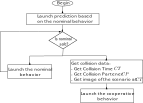
\includegraphics[width=11cm,height=18cm,keepaspectratio]{chapters/Chapitre_6/Figures/STEP1_organi.pdf}
         \caption{Flowchart of the prediction based on the nominal behavior }
         \label{fig:prediction_based_nominal}
         \end{figure}




The image of the merging scenario at CT is used in order to build the list of potential passing sequences. The proposed strategy detects all the potential MVS in-between collisions and classify them in term of riskiness\footnote{The potential collisions are evaluated and classified in terms of their priority. The classification is based on the distance w.r.t. merging zone.}. In Figure \ref{fig:Collision}, the image of the merging scenario at CT, where the virtual projection of the merging vehicle $V_m^{end}$ and the first collision partner $V_{CP_{1}}$ are expected to collide at $t=CT$. 

     \begin{figure}[!h]
        \centering 
        \includegraphics[width=11cm,height=18cm,keepaspectratio]{chapters/Chapitre_6/Figures/Collision.pdf}
        %\vspace{-2.3mm}
        \caption{Image of the merging scenario at $t=CT$ (Collision Time)}
        \label{fig:Collision}
        %\vspace{-5mm}
        \end{figure}





For instance, the list of the potential passing sequences for the scenario in Figure \ref{fig:Collision} can be built as follows: 
\begin{enumerate}
    \item The merging vehicle in-between both of the highway vehicles, $sq(1): V_{CP_1}, \\V_m, V_{hw_2} $
    \item The merging vehicle in front of both of the highway vehicles, $sq(2): V_m,V_{CP_1},\\ V_{hw_2}  $
    \item The merging vehicle in the back of both of the highway vehicles, $sq(3): V_{CP_1}, V_{hw_2},V_m $
\end{enumerate}

In crowded and highly dynamic environment such as the highway, the established list of potential passing sequences can be unsafe. Thus, the potential passing sequence list is augmented with additional potential passing sequences that take into account lane change of the highway vehicles. 

\begin{enumerate}
    \item $V_{CP_1}$ changes lane such as the merging vehicle takes its place, $sq(4): V_{CP_{1_{1\rightarrow 2}}}, V_m, V_{hw_2} $
    \item $V_{CP_2}$ changes lane such as the merging vehicle has enough space to merge, $sq(5): V_{CP_1}, V_m, V_{hw_{2_{1\rightarrow 2}}} $
\end{enumerate}

Once the list of the potential passing sequences is established, it has to be evaluated. The following section is dedicated to draw the details of the selection of the suitable passing sequence. 


\subsection{Suitable passing sequence}\label{sec:suitable_sq}
The suitable passing sequence defines the passing order of the vehicles in the merging zone that solves the collision problem occurred when following the MVS nominal behavior, and that imposes the least changes w.r.t. the MVS nominal dynamics. In other terms, the MVS nominal dynamics are used as a reference dynamics in order to find the closest cooperative behavior to the nominal one, by evaluating the cooperative behavior dynamics that allow to perform safely the potential passing sequence safely.  



 

Figure \ref{fig:negotiation} presents the flowchart of the selection of the passing sequence through an evaluation process. The evaluation of each potential passing sequence is described in Section \ref{sec:global_cooperation_function}, it is based on several quantifiable criteria such as the safety and the dynamics related to the passing sequence. The evaluation focuses also on the altruistic character of the chosen passing sequence. The details of the latter are discussed in Section \ref{sec:altruistic_passing_sequence}. 


    \begin{figure}[!h]
        \centering 
        \includegraphics[width=8cm,height=18cm,keepaspectratio]{chapters/Chapitre_6/Figures/Negotiation.pdf}
        %\vspace{-2.3mm}
        \caption{The flowchart of the MVS passing sequence in the merging zone selection strategy}
        \label{fig:negotiation}
        %\vspace{-5mm}
        \end{figure}




In order to evaluate the performance of the passing sequence selection algorithm, two illustrative scenarios are studied in Section \ref{sec:Simulation_Results}. 



\subsubsection{Global cooperation cost function}\label{sec:global_cooperation_function}
A global cooperation cost function $J_G$ is used to evaluate the level of cooperation related to the different passing sequences $sq$. It uses the initial conditions of the highway vehicles $V_{hw}$ as a reference to define the cooperation effort, and the nominal behavior (cf. Section \ref{sec:The_nominal_mode}) to compare the performance of the merging vehicles $V_m$. It can be written as: 
\begin{align} \label{eq: GlobalCostNegotiation}
    J_{G}(sq(j))= \sum_{i=1}^{N} \omega_{i} J_i  \\
   \sum_{i=1}^{N} \omega_i = 1 \label{eq: sumWeightNegotiation}
\end{align}
%
 $\omega_{i}$ represents the participation weight given to the vehicle $V_{i}$ and it respects the expression given in eq. \ref{eq: sumWeightNegotiation}. $i \in {N} }$ represents the index of the $N$ vehicles part of the considered formation. $J_i$ given in eq. \ref{eq: objectivefunctionnegotiation} is the individual cost function related to each considered vehicle. 

%The cost $J_i$ is given in eq. (\ref{eq: objectivefunctionnegotiation}).% used for the cooperation is composed of four main costs. (a) The cost related to the safety characterized by the inter-vehicular distances. %$J_{i}^{Safe}$. 
%(b) The cost related to the dynamics of the CAV while performing the tackled scenario where it is proposed to deal with the acceleration of the latter,  $J_{i}^{acceleration}$. (c) The cost related to the kinematic energy $J_{i}^{Kinematic Energy}$. The kinematic energy has two objectives: 1) it gives the energy consumption of the CAV even at a constant acceleration. 2) Since it includes the weight of the CAV, it allows a distinction of the efforts asked to be done by a truck and a light-weight CAV. 


%Finally, (d) The Boolean non-collaborative cost $J_{i}^{\substack{ non- \\ collaborative}}$, is designed to avoid exaggerated collaborative scenarios. 

 \begin{align} \label{eq: objectivefunctionnegotiation}
     J_{\substack{ i } = \omega_{safe} J_{i}^{\tiny{Safe}} + \omega_{\tiny{Acc}} J_{i}^{Acc} +\omega_{\tiny{KE}}
     J^{\tiny{KE}} +\omega_{\tiny{\substack{NC}}}J^{\tiny{NC}}, \; \;\;\; \forall i  \in {N}}
 \end{align}
with: 
 \begin{align}
     \omega_{safe} + \omega_{\tiny{Acc}} + \omega_{\tiny{KE}} =1 \\ 
     \omega=\{\omega_{safe}, \omega_{\tiny{Acc}}, \omega_{\tiny{KE}},  \omega_{\tiny{NC}}   \}
 \end{align} 
 %
$\omega$ is the set containing the participation weights given to each sub-cost part of the individual cost $J_{i}$. The non-collaborative weight is used in addition of including non-cooperative vehicle part of the C-MCA, to calibrate the cooperation efforts related to every vehicle. Thus,  $\omega_{NC}$ can only take two states; when the vehicle is said to be cooperative $\omega_{NC}$ is null, in contrast, when the vehicle is said to be not cooperative $\omega_{NC}$ is equal to big value, allowing to not consider the corresponding solution. The cost $J_i$ is composed of the four components described above: 
 
 
 
\begin{enumerate}[(a)]

%%%%%the distance cost 
\item The safety related cost $J_{i}^{Safe}$ considers the Euclidean inter-vehicular distances in between the vehicles part of the formation. It can be written as in eq. \ref{eq:SafetyNegotiation}: 

\begin{equation}\label{eq:SafetyNegotiation}
J_{i}^{Safe} = \frac{\sum_{k=1}^{I_S}\frac{1}{EucDist\{X_{V_{i}}(k), X_{V_{j}}(k)\}^{\forall j \in  {N}, j\neq i}}}{\sum_{k=1}^{I_S}\frac{1}{d_{Safe}}}, \; \;\;\; \forall i  \in {N}}
    \end{equation}

$d_{safety}$ is the safety distance that needs to be always respected between the vehicles. It corresponds to twice the radius of the safety circle around the vehicle (cf. Figure \ref{fig:Collision}). The latter is chosen to take into account the dimensions of the vehicle in addition of a certain offset. $I_S$ represented the time samples needed to perform the merging with the help of the cooperative behavior. It is used here to normalize the safety cost.





%%% the acceleration cost 



\item The cost related to the dynamics of the vehicles $J_{m}^{Acc}$ utilizes the acceleration. This cost  aims to minimize the gap between the nominal dynamic and the cooperation-based dynamic related to $V_m, \; \forall m \in \mathbb{M}$. The subset $\mathbb{M}$ with $\mathbb{M} \in {N}$ contains only the $m$-indexes of the merging vehicles $V_m$ (cf. Figure \ref{fig:Collision}). 

\begin{equation}
       J_{\substack{ m }}^{Acc}= \Big\lvert \frac{1}{I_{N}} \sum_{k=1}^{I_{N}} \Big[ \frac{a^{nominal}_{m}(k)}{\overline{a^{nominal}_{m}}}\Big]^2 -   \frac{1}{I_{S}}  \sum_{k=1}^{I_S} \Big[ \frac{a^{S}_{m}(k)}{\overline{a^{S}_{m}}}\Big]^2 \Big\rvert, \; \; \; \forall \, m  \in \mathbb{M}}
\end{equation}



As for the highway vehicles $V_{hw}$, their dynamics are represented with the cost $J_{\substack{ hw }}^{Acc}, \; \; \;  \forall \, hw  \in \mathbb{H}}$. The subset $\mathbb{H}$ with $\mathbb{H} \in {N}$ contains only the $hw$-indexes of the highway vehicles $V_{hw}$ (cf. Figure \ref{fig:Collision}). 

\begin{align}
    J_{\substack{ hw }}^{Acc} =  \frac{1}{I_{S}}  \sum_{k=1}^{I_S} \Big[ \frac{a^{S}_{hw}(k)}{\overline{a^{S}_{hw}}}\Big]^2 , \; \; \; \forall \, hw  \in \mathbb{H}
\end{align}

with $a_{m}^{S}$ and $a_{hw}^{S}$ being respectively,  the acceleration profile of the $V_m$ and $V_{hw}$ during the merging scenario under the cooperation behavior. $\overline{a^{nominal}_{m}}$ and $\overline{a^{S}_{m}}$ are the maximum acceleration with the nominal behavior (cf. Section \ref{sec:The_nominal_mode}) and with the cooperation behavior, respectively. The latter are used to normalize the acceleration cost.




\item The cost related to the energy generated by the cooperative behavior is characterized by the kinetic energy used by the vehicles (cf. eq. \ref{eq: kinematicEnegyMergingCost} and eq. \ref{eq: kinematicEnegyHighwayCost}).  The kinetic energy related cost has two objectives: 1) It gives the energy consumption of the vehicle even at zero acceleration. 2) Since it includes the weight of the vehicle, it allows for instance the distinction of the efforts asked to be done by a truck and a light-weight vehicle. 

Same as for the dynamic related cost, the nominal dynamic (cf. Section \ref{sec:The_nominal_mode}) is used to evaluate and minimize the gap between the nominal behavior dynamic and the cooperation one. Thus, the kinetic energy cost for the merging vehicle is shown in eq. \ref{eq: kinematicEnegyMergingCost}.
\begin{equation}\label{eq: kinematicEnegyMergingCost}
    J_{\substack{ m }}^{\tiny{KE}} = \frac{1}{2} m_{V_{m}} \Big\lvert \frac{1}{I_{N}} \sum_{k=1}^{I_{N}} \Big[ \frac{\mathcal{V}^{nominal}_{m}(k)}{\overline{\mathcal{V}^{nominal}_{m}}}\Big]^2 -   \frac{1}{I_{S}}  \sum_{k=1}^{I_S} \Big[ \frac{\mathcal{V}^{S}_m(k)}{\overline{\mathcal{V}^{S}_m}}\Big]^2 \Big\rvert , \; \; \; \forall m  \in \mathbb{M}
\end{equation}
 The kinetic energy related to the highway vehicles is noted $J^{\tiny{KE}}_{hw}$ and it is given in eq. \ref{eq: kinematicEnegyHighwayCost}. 
 
\begin{flalign} \label{eq: kinematicEnegyHighwayCost}
    J_{\substack{ hw }}^{\tiny{KE}} =  \frac{1}{2} m_{V_{hw}} \Big(\frac{1}{I_{S}}  \sum_{k=1}^{I_S} \Big[ \frac{\mathcal{V}_{ref}^{S}(k)- \mathcal{V}^{S}_{hw}(k)} {\tiny{max}({\overline{\mathcal{V}_{ref}^{S}}, \overline{\mathcal{V}^{S}_{hw}}})}\Big]^2\Big) , \; \; \; \forall hw  \in \mathbb{H}
\end{flalign}


with $m_{V_{i}}$ being the weight of the vehicle $V_i$. $\mathcal{V}_{m}^{S}$ and $\mathcal{V}_{hw}^{S}$ are the velocity profiles of both $V_m$ and $V_{hw}$, respectively,  during the merging scenario under the cooperation behavior. $\mathcal{V}_{ref}^S$ is the desired velocity of the $V_{hw}$. The term ${\tiny{max}({\overline{\mathcal{V}_{ref}^{S}}, \overline{\mathcal{V}^{S}_{hw}}})}$ is used for the normalization of the kinetic energy cost.




\subsubsection{Altruistic passing sequence}\label{sec:altruistic_passing_sequence}
The fourth term of the individual cost function is the non-collaborative cost. Its objective is to ensure the avoidance of extensive cooperation efforts from the perspective of the V$_{hw}$. In fact, the highway MVS are said to be altruistic, in other terms, they are set as collaborative by definition. However, the  cost in eq. \ref{eq:non_cop_omega} plays the role of the cooperation threshold from the $V_{hw}$ perspective. The threshold represents the maximum cooperation tolerance of the highway vehicle. Consequently, when a passing order $sq$ orders the $V_{hw_i}$ an effort above its effort's threshold, the non-collaborative cost is maximized.

\begin{equation} \label{eq:non_cop_omega}
    \omega_{NC} = \left\{ \begin{array}{rcl}
0 & \mbox{for}
& J_{NC}< threshold \\ 
\inf & \mbox{for} & J_{NC}  \geq threshold
\end{array}\right.
\end{equation}

 The non-collaborative cost $J_{NC}$ represents the highway vehicle cooperation effort. In fact, the nominal behavior is said to be the best behavior, thus, $J_{NC}$ aims to quantify the gap separating the dynamics imposed by the cooperative behavior in comparison to the nominal ones.  The non-cooperative cost  $J_{NC}$ is given in equation in eq. \ref{eq: non_collaboration cost}. 

\begin{equation} \label{eq: non_collaboration cost}
    J_{NC}= \abs{\frac{J_{cooperation}-J_{nominal}}{J_{nominal}}}
\end{equation}

with $J_{cooperation}$ and $J_{nominal}$ being the cooperation-related and the nominal-related costs, respectively. Both of the costs are given in eq. \ref{eq:nominal_cost} and eq. \ref{eq:cooperation_cost}, respectively. 

\begin{equation}\label{eq:nominal_cost}
    J_{nominal}= \sum _{k=1}^{I_N} \frac{\mathcal{V}(k)_{nominal}}{\overline{\mathcal{V}_{nominal}}} + \sum _{k=1}^{I_N} \frac{a (k)_{nominal} }{\overline{a}_{nominal}}}
\end{equation}


\begin{equation}\label{eq:cooperation_cost}
    J_{cooperation}= \sum _{k=1}^{I_S} \frac{\mathcal{V}(k)_{cooperation}}{\overline{\mathcal{V}_{cooperation}}} + \sum _{k=1}^{I_S} \frac{a (k)_{cooperation} }{\overline{a}_{cooperation}}}
\end{equation}

where $\{\mathcal{V}_{nominal}, a_{nominal}\}$ are the velocity and the acceleration profile generated by the nominal behavior, and $\{\overline{\mathcal{V}_{nominal}}, \overline{a_{nominal}}\}$ are their maximum values. $\{\mathcal{V}_{cooperation}, a_{cooperation}\}$ are the velocity and the acceleration profile generated by the cooperative behavior, and $\{\overline{\mathcal{V}_{cooperation}}, \overline{a_{cooperation}}\}$ are their maximum values. 
 \end{enumerate}





\section{Simulation results}\label{sec:Simulation_Results}
The proposed decision-making level part of C-MCA was designed to select the appropriate behavior of the MVS when performing the merging. As stated above, two behaviors are implemented in the C-MCA, so that the MVS prioritize a nominal merging maneuver when possible. If needed, the MVS is expected to cooperate in order to overcome the collision risk related to the merging, without neglecting the dynamics of the vehicles part of it. 

In this section it is proposed through two illustrative scenarios to study and evaluate the decision chosen by the decision-making level. Thus, the C-MCA is asked to solve both scenarios, as well as to evaluate the solution through the prism of the safety, feasibility and energy efficiency related to the MVS. The simulations were conducted using Matlab/Simulink and SCANeR studio simulator \ref{sec:SCANeR-studio}. 

The first scenario aims to test the C-MCA ability to solve a conflicting on-ramp merging on highway. Based on the passing sequence selected by the decision-making level, the E-CORM is tasked to generate the required MVS dynamics needed w.r.t. the passing sequence. The details and the results related to this first scenario are presented in this section. 

In addition to find a suitable solution, the C-MCA needs to assess the safety criterion and when needed, online resolve conflicting scenarios. The second scenario was built to test this particularity. Thus, with the help of the cooperative optimization free formation reconfiguration framework seen in Section \ref{sec:No-opt}, a dynamic scenario is proposed where the C-MCA performed the merging safely. 

\subsection*{Scenario 1}
The following simulation presents an on-ramp merging on highway performed by four vehicles (three highway vehicles $V_{hw_1}$, $V_{hw_2}$, $V_{hw_3}$ and the merging vehicle $V_{m}$) being part of the MVS (cf. Figure \ref{fig:scenario01:scenario_scene}). In order to study the C-MCA ability to solve conflicting mergings, the MVS vehicles are placed in positions where the safety criterion is triggered (cf. Figure \ref{fig:scenario01:scenario_scene}). Thus, the cooperation behavior is activated in order to solve the conflict occurred in the merging zone. The simulation video related to this scenario can be found in \textcolor{blue}{https://shorturl.at/gjGKL}. 







     \begin{figure}[!h]
        \centering 
        \includegraphics[width=13cm,height=18cm,keepaspectratio]{chapters/Chapitre_6/Figures/Scenario_1/Scenario_scene.pdf}
        %\vspace{-2.3mm}
        \caption{Scenario 1: Illustration of the on-ramp merging on highway scene. The initial shape of the formation under the communication range of the RSU is represented, along with the desired shape }
        \label{fig:scenario01:scenario_scene}
        %\vspace{-5mm}
        \end{figure}


Figure \ref{fig:scenario01:formation_shape} (b.1) shows the formation shape when the merging is being performed by the nominal behavior. In fact, a collision is detected between the merging vehicle and the highway vehicle at $t=3.6s$. Consequently, the cooperative behavior is asked to solve the predicted collision. Thus, a list of potential passing sequences was built. In Table \ref{Tab: Summary_scenario_01}  the results of the best passing sequence is shown. 



     \begin{figure}[!h]
        \centering 
        \includegraphics[width=13cm,height=18cm,keepaspectratio]{chapters/Chapitre_6/Figures/Scenario_1/Fromation_shape.pdf}
        %\vspace{-2.3mm}
        \caption{Evolution of the formation' shape during the on-ramp merging on highway}
        \label{fig:scenario01:formation_shape}
        %\vspace{-5mm}
        \end{figure}




\begin{table}[!h]
\setlength\tabcolsep{6pt} % default value: 6pt

%\scriptsize{}

\caption{Scenario 1: Numerical results of the cooperation behavior }
%\vspace{-3mm}
\label{Tab: Summary_scenario_01}
\begin{tabular}{|l|ccccl|ccccl|}
\hline
sq                 & \multicolumn{5}{c|}{V$_{hw_1}$,V$_{hw_2}$,V$_{hw_3}$,V$_{m}$}                                                                          & \multicolumn{5}{c|}{V$_{hw_1}$,V$_{hw_2}$,V$_{m}$,V$_{hw_3}$}                                                                          \\ \hline
J$_{G} $           & \multicolumn{5}{c|}{\textbf{0.1159}}                                                                                  & \multicolumn{5}{c|}{0.1642}                                                                                           \\ \hline
Vehicle id                & \multicolumn{1}{c|}{$_{hw_1}$}     & \multicolumn{1}{c|}{$_{hw_2}$}     & \multicolumn{1}{c|}{$_{m}$}     & \multicolumn{2}{c|}{$_{hw_3}$}     & \multicolumn{1}{c|}{$_{hw_1}$}     & \multicolumn{1}{c|}{$_{hw_2}$}     & \multicolumn{1}{c|}{$_{m}$}     & \multicolumn{2}{c|}{$_{hw_3}$}     \\ \hline
J$^{safe}$       & \multicolumn{1}{c|}{0.0705} & \multicolumn{1}{c|}{0.0884} & \multicolumn{1}{c|}{0.1058} & \multicolumn{2}{c|}{0.1031} & \multicolumn{1}{c|}{0.0871} & \multicolumn{1}{c|}{0.0894} & \multicolumn{1}{c|}{0.1451} & \multicolumn{2}{c|}{0.1031} \\ \hline
J$^{acc}$ & \multicolumn{1}{c|}{0}      & \multicolumn{1}{c|}{0}      & \multicolumn{1}{c|}{0.1290} & \multicolumn{2}{c|}{0.0571} & \multicolumn{1}{c|}{0}      & \multicolumn{1}{c|}{0}      & \multicolumn{1}{c|}{0.1188} & \multicolumn{2}{c|}{0.0971} \\ \hline
J$^{KE} $      & \multicolumn{1}{c|}{0}      & \multicolumn{1}{c|}{0}      & \multicolumn{1}{c|}{0.0574} & \multicolumn{2}{c|}{0.1159} & \multicolumn{1}{c|}{0}      & \multicolumn{1}{c|}{0}      & \multicolumn{1}{c|}{0.1405} & \multicolumn{2}{c|}{0.1509} \\ \hline
\end{tabular}
\vspace{-3mm}
\end{table}


Several passing sequences were tested and evaluated in terms of their safety, comfort and energy efficiency. The passing sequence selected by the cooperation behavior is $sq=\{V_{hw_1}, V_{hw_2}, V_{hw_3}, V_{m}\}$ (cf. Table \ref{Tab: Summary_scenario_01}). Figure \ref{fig:scenario01:formation_shape} (b.2) shows the formation shape when merging vehicle enters the merging zone at $t=3.6s$. It can noticed that the selected passing sequence has solved the collision occurred when following the nominal behavior. In Figure \ref{fig:scenario01:formation_shape} (c), the formation shape at the end of the merging maneuver is illustrated, where the MVS follows a platoon-based formation shape as expected. 









  














 

The Euclidean distances within the MVS are given in Figure \ref{fig:scenario01:formation_distances}, where conflict between the merging vehicle V$_m$  and the highway vehicle $V_{hw_3}$ can be noticed around $t=3.6s$ (cf. Figure \ref{fig:scenario01:formation_distances}, in dashed magenta). Thanks to the cooperation behavior part of the C-MCA, the conflict is solved, where the Euclidean distance between $V_m$ and $V_{hw_3}$ is always greater than the minimum allowed safety distance (cf. Figure \ref{fig:scenario01:formation_distances}, in blue plot). 

    \begin{figure}[!h]
        \centering 
        \includegraphics[width=13cm,height=18cm,keepaspectratio]{chapters/Chapitre_6/Figures/Scenario_1/Distances.pdf}
        %\vspace{-2.3mm}
        \caption{Euclidean in-between distances within the formation}
        \label{fig:scenario01:formation_distances}
        %\vspace{-5mm}
        \end{figure}

The overall MVS reconfiguration during the merging  respects the safety criterion, since the rest of the vehicles Euclidean in-between distances are all greater than the minimum safety distance. 







 The velocity profiles of the vehicles corresponding to the selected passing sequence $sq$ (cf. Table \ref{Tab: Summary_scenario_01}) are depicted in Figure \ref{fig:scenario01:formation_velocity} (a). The velocity profiles respect the maximum authorized velocity ($80 \; km/h$ in segment A and $130 \; km/h$ in segment B). Since the highway vehicle $V_{hw_3}$ is expected to be ahead of the merging vehicle, it has to accelerate in order to reduce its spacing w.r.t. $V_{hw_2}$. The merging vehicle has a lower initial velocity in comparison to the highway vehicles. Consequently, it has to accelerate, while respecting the authorized maximum velocity in each traveled segment, in order to respect the selected passing sequence $sq$. The final velocity of the MVS corresponds to the reference vehicle $V_{hw_1}$ velocity in order to be able to maintain the desired platoon shape with equal in-between distances. The overall acceleration profiles respect the maximum and minimum authorized limits (cf. Figure \ref{fig:scenario01:formation_velocity} (b)).
     \begin{figure}[!h]
        \centering 
        \includegraphics[width=9cm,height=18cm,keepaspectratio]{chapters/Chapitre_6/Figures/Scenario_1/Velocity.pdf}
        %\vspace{-2.3mm}
        \caption{The vehicles' velocity and acceleration profiles}
        \label{fig:scenario01:formation_velocity}
        %\vspace{-5mm}
        \end{figure}








\newpage
\subsection*{Scenario 2}
The goal of this scenario is to evaluate the capacity of the C-MCA to access the safety criterion of the MVS during the merging maneuver, while being able to solve online conflicting situation when occurred. Consequent, an unforeseen event is introduced to the studied scenario at $t=8s$. The scenario is divided into two part, the first part is related to the merging scenario before $t=8s$, while the second part focuses on the effects of the unexpected introduced event and its begins after $t=8s$. The simulation video can be found in \textcolor{blue}{https://youtu.be/u0LRJbOW94M}.

The scenario in figure \ref{fig:scenario02:scenario_scene} uses a formation of five vehicles that participate into the on-ramp merging on highway. The initial position of the merging vehicle $V_m$ is configured to trigger the safety criterion part of the proposed C-MCA, in Figure \ref{fig:scenario02:formation_shape} (a) Initial shape of the formation, the initial vehicles positions are illustrated with the help of the snapshot from the SCANeR studio engine. Consequently, it is the cooperative behavior that will generate the vehicles' dynamics in order to perform the merging maneuver. In Table \ref{Tab:scenario2.1}, the numerical results of the cooperative behavior are shown. The $sq=\{V_{hw_{1}},V_{hw_{2}},V_{m},V_{hw_{3}}\}$ is the best passing sequence according to the cooperative behavior (cf. Section \ref{sec:Cooperative_mode}). 




   \begin{figure}[!h]
        \centering 
        \includegraphics[width=13cm,height=18cm,keepaspectratio]{chapters/Chapitre_6/Figures/Scenario_2/Scenario2_ScenarioScene.pdf}
        %\vspace{-2.3mm}
        \caption{Scenario 2: Illustration of the on-ramp merging on highway scene. The initial shape of the formation under the communication range of the RSU is represented, along with the desired shape (\textcolor{blue}{Simulation video: https://youtu.be/u0LRJbOW94M})}
        \label{fig:scenario02:scenario_scene}
        %\vspace{-5mm}
        \end{figure}














     \begin{figure}[!h]
        \centering 
        \includegraphics[width=14cm,height=18cm,keepaspectratio]{chapters/Chapitre_6/Figures/Scenario_2/Formation_Reconfiguration_Scenario2.pdf}
        %\vspace{-2.3mm}
        \caption{Illustrative snapshots obtained from the SCANeR studio engine presenting the evolution of the formation during the merging maneuver}
        \label{fig:scenario02:formation_shape}
        %\vspace{-5mm}
        \end{figure}













\begin{table}[!h]
\setlength\tabcolsep{6.0pt} % default value: 6pt

%\scriptsize{}
%\centring
\caption{Scenario 2.1: Numerical results of the cooperation behavior before $t=8s$}
%\vspace{-3mm}
\label{Tab:scenario2.1}
\begin{tabular}{|c|cccc|cccc|}
\hline
$sq$       & \multicolumn{4}{c|}{$V_{hw_{1}},V_{m},V_{hw_{2}},V_{hw_{3}}$}                                                       & \multicolumn{4}{c|}{$V_{hw_{1}},V_{hw_{2}},V_{m},V_{hw_{3}}$}                                                       \\ \hline
$J_G$      & \multicolumn{4}{c|}{0.196}                                                                   & \multicolumn{4}{c|}{{\textbf{0.181}}}                                                 \\ \hline
Vehicle id    & \multicolumn{1}{c|}{hw_{1}}     & \multicolumn{1}{c|}{m}     & \multicolumn{1}{c|}{hw_{2}}     & hw_{3}     & \multicolumn{1}{c|}{hw_{1}}     & \multicolumn{1}{c|}{m}     & \multicolumn{1}{c|}{hw_{2}}     & hw_{3}         \\ \hline
$J^{safe}$ & \multicolumn{1}{c|}{0.125} & \multicolumn{1}{c|}{0.15}  & \multicolumn{1}{c|}{0.103} & 0.066 & \multicolumn{1}{c|}{0.109} & \multicolumn{1}{c|}{0.25}  & \multicolumn{1}{c|}{0.227} & 0.063 \\ \hline
$J^{acc}$  & \multicolumn{1}{c|}{0}     & \multicolumn{1}{c|}{0.11}  & \multicolumn{1}{c|}{0.047} & 0.063 & \multicolumn{1}{c|}{0}     & \multicolumn{1}{c|}{0.335} & \multicolumn{1}{c|}{0.025} & 0.035 \\ \hline
$J^{KE}$  & \multicolumn{1}{c|}{0.127} & \multicolumn{1}{c|}{0.586} & \multicolumn{1}{c|}{0.292} & 0.292 & \multicolumn{1}{c|}{0.127} & \multicolumn{1}{c|}{0.102} & \multicolumn{1}{c|}{0.11}  & 0.147 \\ \hline
\end{tabular}
%\vspace{-5mm}
\end{table}



\newpage



However, around $t=8s$, the fifth vehicle decides to join the formation (cf. Figure \ref{fig:scenario02:formation_shape} (b)). As a result, the initial passing sequence no longer satisfies the safety requirement, prompting the cooperative behavior to recalculate a suitable $sq$ to ensure safe reconfiguration. Four passing sequences were considered by the cooperative behavior part of the C-MCA. In Table \ref{Tab: Scenario2.2}, the numerical results of the two best $sq$ are presented. 


\begin{table}[!h]
\setlength\tabcolsep{6pt} % default value: 6pt

%\scriptsize{}
%\centring
\caption{Scenario 2.2: Numerical results of the cooperation behavior after $t=8s$}
%\vspace{-3mm}
\label{Tab: Scenario2.2}

\begin{tabular}{|c|ccccl|ccccl|}
\hline
$sq$       & \multicolumn{5}{c|}{$V_{hw_{1}},V_{hw_{2}},V_{m},V_{hw_{4}}, V_{hw_3}$}                                                                                    & \multicolumn{5}{c|}{$V_{hw_1},V_{hw{2_{1\rightarrow2}}},V_m,V_{hw_4}, V_{hw_3}$}                                                                              \\ \hline
$J_G$      & \multicolumn{5}{c|}{0.267}                                                                                                & \multicolumn{5}{c|}{{\textbf{0.242}}}                                                                              \\ \hline
Vehicle  id    & \multicolumn{1}{c|}{hw_{1}}     & \multicolumn{1}{c|}{m}     & \multicolumn{1}{c|}{hw_{2}}     & \multicolumn{1}{c|}{hw_{3}}      & hw_{4}      & \multicolumn{1}{c|}{hw_{1}}     & \multicolumn{1}{c|}{m}     & \multicolumn{1}{c|}{hw_{2}}     & \multicolumn{1}{c|}{hw_{3}}       & hw_{4}      \\ \hline
$J^{safe}$ & \multicolumn{1}{c|}{0.104} & \multicolumn{1}{c|}{0.358} & \multicolumn{1}{c|}{0.227} & \multicolumn{1}{c|}{0.085} & 0.011 & \multicolumn{1}{c|}{0.101} & \multicolumn{1}{c|}{0.185} & \multicolumn{1}{c|}{0.129} & \multicolumn{1}{c|}{0.106} & 0.017 \\ \hline
$J^{acc}$  & \multicolumn{1}{c|}{0}     & \multicolumn{1}{c|}{0.11}  & \multicolumn{1}{c|}{0.135} & \multicolumn{1}{c|}{0.035} & 0.041 & \multicolumn{1}{c|}{0}     & \multicolumn{1}{c|}{0.156} & \multicolumn{1}{c|}{0.089} & \multicolumn{1}{c|}{0.031} & 0.152 \\ \hline
$J^{KE}$  & \multicolumn{1}{c|}{0.127} & \multicolumn{1}{c|}{0.402} & \multicolumn{1}{c|}{0.188} & \multicolumn{1}{c|}{0.147} & 0.152 & \multicolumn{1}{c|}{0.127} & \multicolumn{1}{c|}{0.262} & \multicolumn{1}{c|}{0.136} & \multicolumn{1}{c|}{0.153} & 0.148 \\ \hline
\end{tabular}
\end{table}

The $sq={V_{hw_1},V_{hw{2_{1\rightarrow2}}},V_m,V_{hw_4}, V_{hw_3}}$ is the best passing sequence. The $V_{hw_2}$ is asked to change the lane from $lane \,1$ to $lane \,2$ (cf. Figure \ref{fig:scenario02:formation_shape} (c) Formation shape at the merging zone). The simulation results obtained following the selected $sq$ are presented in the following figures.

In Figure \ref{fig:scenario02:formation_coordinates}, the longitudinal and the lateral coordinates of the formation are presented. The green shaded part is related to the merging vehicle traveling in segment A, while the red shaded part related to the segment B. The inclusion of the fifth vehicle at $t=8s$ stimulated the reactivity of the C-MCA, leading to a switch in the configuration at $t=8s$ (cf. Figure \ref{fig:scenario02:formation_coordinates}). The continuity of the reconfiguration is ensured formally by the optimization-free formation reconfiguration framework presented in Section \ref{sec:No-opt}. The selected $sq$ requires a lane change of $V_{hw_2}$, what can be seen in its lateral coordinate plot. The merging vehicle exits the merging road to join the highway desired lane according to its lateral coordinate plot. The desired shape of the formation is a platoon formation for the vehicles traveling on the same lane with equal spacing w.r.t. the reference vehicle $V_{hw_1}$. 



     \begin{figure}[!h]
        \centering 
        \includegraphics[width=8cm,height=18cm,keepaspectratio]{chapters/Chapitre_6/Figures/Scenario_2/coordi_s2.pdf}
        %\vspace{-2.3mm}
        \caption{Formation coordinates during the on-ramp merging on highway}
        \label{fig:scenario02:formation_coordinates}
        %\vspace{-5mm}
        \end{figure}




The Euclidean in-between distances are presented in Figure \ref{fig:scenario02:formation_distances}. The highway vehicle $V_{hw_2}$ and the merging vehicle travel in two different lanes in the desired formation shape, but placed according to the same longitudinal coordinate w.r.t. the reference vehicle $V_{hw_1}$. Consequently, the Euclidean distance between these two vehicles is above $d_{safe}$, due to the existence of only the lateral separation (two different lanes). The rest of the Euclidean distances are all greater than $d_{safe}$, thus the merging can be considered as a safe maneuver. 


     \begin{figure}[!h]
        \centering 
        \includegraphics[width=13cm,height=18cm,keepaspectratio]{chapters/Chapitre_6/Figures/Scenario_2/Scenario2_distances.pdf}
        %\vspace{-2.3mm}
        \caption{The Euclidean in-between distances}
        \label{fig:scenario02:formation_distances}
        %\vspace{-5mm}
        \end{figure}

        
The velocity profiles of the vehicles part of the MVS performing the merging are displayed in Figure \ref{fig:scenario02:formation_velocity}. As can be seen, the formation switch at $t=8s$ created a dynamic switch in the merging vehicle velocity profile. The rest of the vehicles' velocity profiles respect the maximum authorized velocity in the traveled segment. 
     \begin{figure}[!h]
        \centering 
        \includegraphics[width=13cm,height=18cm,keepaspectratio]{chapters/Chapitre_6/Figures/Scenario_2/Scenario2_velocity.pdf}
        %\vspace{-2.3mm}
        \caption{The vehicles' velocity profiles}
        \label{fig:scenario02:formation_velocity}
        %\vspace{-5mm}
        \end{figure}
 
\section{Conclusion}

 



This chapter has provided an in-depth exploration of the multi-behavior decision-making strategy within the proposed C-MCA. The decision-making strategy is structured around two distinct behaviors:

 \begin{itemize}
     \item The nominal behavior:   This behavior is specifically crafted to execute the merging maneuver while ensuring the fulfillment of individual vehicle goals.

     \item The cooperative behavior:    Activated by the decision-making level when the safety requirement is not met by the nominal behavior, the cooperative behavior aims to address merging conflicts by generating a safe passing sequence. The particularity of the generated passing sequence lies in the selection process governing its generation. Notably, the cooperative behavior is proposed to produce MVS dynamics that maintain the satisfaction of individual vehicle goals, while solving the merging conflict. Thanks to the altruistic passing sequence selection strategy  that permits to exclude the passing sequence that do not meet the vehicle's individual goals. 
 \end{itemize}


The performance of the proposed multi-behavior decision-making strategy was evaluated through simulation scenarios, where both of the nominal and the cooperative behavior have been activated. 



